\documentclass{beamer}
\usetheme{Darmstadt}
\usecolortheme{beaver}
\usepackage{booktabs}
\usepackage{hyperref}

\usepackage[utf8]{inputenc}
\usepackage{graphicx}
\graphicspath{ {./images/} }

%Information to be included in the title page:
\title{Homework 03}
\author{Brandon Hosley}
\institute{University of Illinois - Springfield}
\date{\today}

\begin{document}
\frame{\titlepage}

\begin{frame}{Overview}
\tableofcontents
\end{frame}

\section[Q1]{Q1: Linear Regression}

\begin{frame}{Linear Regression Problem 1: Simplicity}
	\begin{itemize}
		\item[+] Computationally easy
		\item[-] Can only accurately represent simple relationships
		\item[-] Can only accurately represent linear relationships
	\end{itemize}
	\includegraphics[width=0.75\linewidth]{AnscombeQuartet}
\end{frame}

\begin{frame}{Linear Regression Problem 2: Selection Bias}
	Linear regression is susceptible to selection bias
	\begin{itemize}
		\item A type of overfitting
		\item Occurs when a type of data is over-represented in test set
	\end{itemize}
	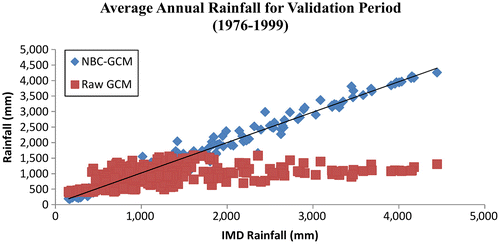
\includegraphics[width=0.45\linewidth]{SelectionBias}
	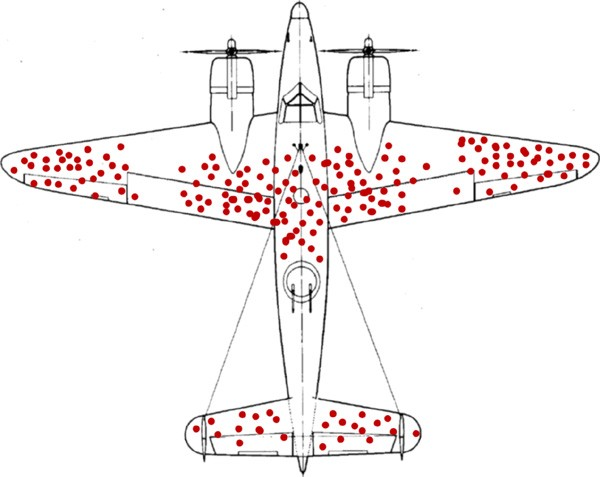
\includegraphics[width=0.45\linewidth]{SelectionAnecdote}
\end{frame}

\begin{frame}{Linear Regression Problem 3: Multicolinearity}
	\begin{itemize}
		\item When multiple predictors share a linear relationship
		\item Small changes are magnified in the model
		\item Heavily correlated predictors may cause redundancy in model
	\end{itemize}
	\includegraphics[width=0.75\linewidth]{Multicolinearity}
\end{frame}

\begin{frame}{Linear Regression Problem 4: Heteroscedasticity}
	\begin{itemize}
		\item Divergent data
		\item May be easily bound between two curves
		\item Difficult to accurately predict 
	\end{itemize}
	\centering
	\includegraphics[width=0.5\linewidth]{Heteroscedasticity}
\end{frame}

\section[Q2]{Q2: Hastie and Tibshirani Summary}

\begin{frame}{Tibshirani Lecture: Linear Regression}
	\begin{itemize}
		\item<1-> Linear Regression
		\begin{itemize}
			\item<1-> Simple approximation method
			\item<1-> Great for estimating slope of data
			\item<1-> From this one may generate confidence interval
		\end{itemize}
		\item<2> Hypothesis Testing
		\begin{itemize}
			\item<2> Testing against a null hypothesis
			\item<2>[] $H_0$ : No relationship between $X$ and $Y$.
			\item<2> Testing for the probability of independent variable distribution 
		\end{itemize}
	\end{itemize}
	\only<1>{\includegraphics[width=0.75\linewidth]{ConfidenceIntervals}}
	\only<2>{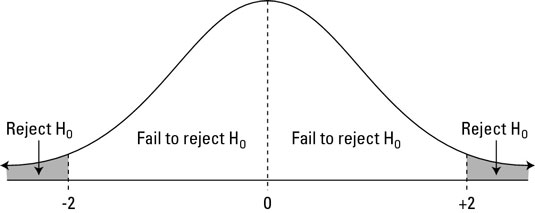
\includegraphics[width=0.75\linewidth]{nullHypothesis}}
\end{frame}

\begin{frame}{Tibshirani Lectures: Multiple Linear Regression}
\begin{columns}
	\column{0.5\textwidth}
	\begin{itemize}
		\item<1-> Multiple Linear Regression
		\begin{itemize}
			\item<1-> Fitting data to a hyperplane instead of line
			\item<1-> Works best when variables are independent
		\end{itemize}
	\end{itemize}
	\column{0.5\textwidth}
	\only<1>{\includegraphics[width=0.75\linewidth]{hyperplane}}
\end{columns}	
\end{frame}

\begin{frame}{Tibshirani Lectures: Choosing Variables}
	\begin{itemize}
		\item<1-> Selection from all subsets
		\item<1-> Forward Selection - adding variables with highest significance
		\item<1-> Backward Selection - removing variables with least significance
	\end{itemize}
	%\only<1>{\includegraphics[width=0.75\linewidth]{hyperplane}}	
\end{frame}

%\section[Q3]{Q3: ISL Section 3.6}
%\section[Q4]{Q4: ISL Section 3.7}
%Exercises. No. 15

\end{document}
